\chapter{The sPHENIX Project}
\label{chap:project}

The sPHENIX detector is being realized via several projects that are
coordinated under a common project management structure.  There are
the elements of the original DOE MIE --- the 1.5~T BaBar
superconducting solenoid, the outer hadronic calorimeter (oHCal), the
central rapidity portion of electromagnetic calorimeter (EMCal)
covering $|\eta| < 0.85$, the time projection chamber (TPC), and their
associated readout electronics and services.  A silicon strip tracker
(INTT) is being provied by RIKEN.  Additional tungsten/scintillating
fiber blocks extending the coverage of the EMCal to $|\eta| < 1.1$ are
being provided by a consortium of Chinese collaborating institutions.
The inner longitudinal section of the hadronic calorimeter (iHCal) and
the silicon pixel vertex detector (MVTX) are being pursued as BNL
capital projects.  A quartz \v{C}erenkov minimum bias detector,
originally built by Hiroshima University for the PHENIX experiment, is
being repurposed for use in sPHENIX.  There are also BNL funded
projects to upgrade the infrastructure at IP8 and to integrate and
install the sPHENIX detector into the IP.  A labeled depiction of the
sPHENIX detector can be seen in Fig.~\ref{fig:sPHENIX}.

\section{Project timeline}
\label{sec:timeline}

The sPHENIX MIE received CD-1/3A approval in August 2018.  A memo from
DOE that saeme summer specified that project with a TPC below \$50M
would no longer be managed under DOE Order 413.3B, but would instead
be managed by a process, the details of which were to be worked out
between the National Laboratorie and DOE.  The result was that sPHENIX
would be working toward Project Decisions (PDs), to be approved by the
BNL Laboratory Director with DOE concurrence.  sPHENIX received PD-2/3
approval in September 2019.

\section{Elements of the Project}
\label{sec:elements}

The full sPHENIX project consists of a large number of different
elements.  The 600 ton detector will be supported by a steel structure
on a platform on a rail system.  The magnetic flux of the
superconducting solenoid will be returned in part by steel end cap
doors.  A set of platforms, accessed by stairs, will support
electronic racks and the cryogenic services for the solenoid.  See
Fig.~\ref{fig:sPHENIX}.

The detector nearest the collision point is the MVTX, a silicon pixel
detector closely based on the ALICE ITS inner barrel.  See
Fig.~\ref{fig:mvtx}.  The MVTX is capable of 5~$\mu m$ resolution for
tracks with $p_T > 1$~GeV/c and enables the open heavy flavor program.

\begin{figure}[hbt!]
  \centering
  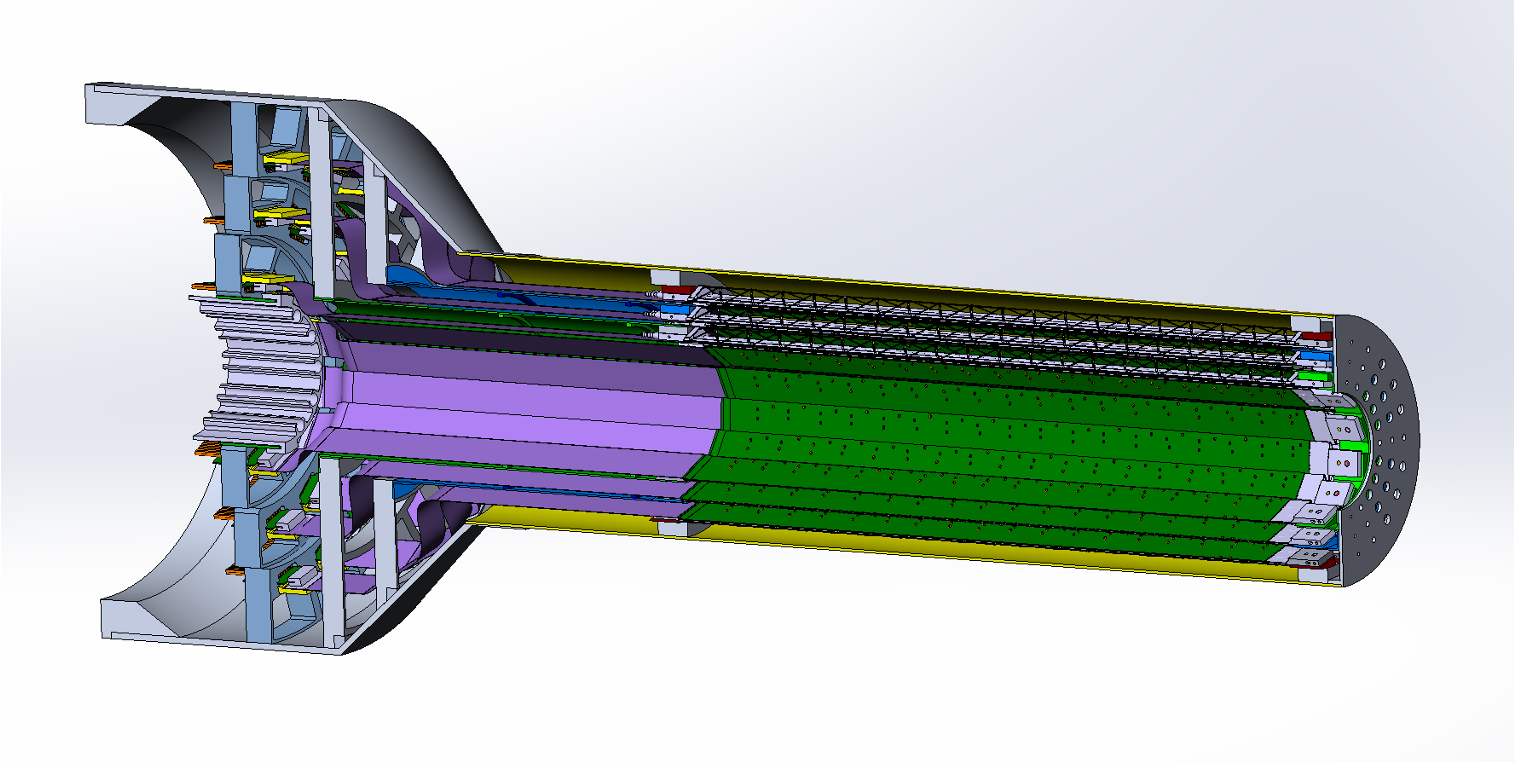
\includegraphics[width=0.9\linewidth]{mvtx_oblique}
  \caption{A rendering of a half barrel of the MVTX in its carbon
    fiber support structure.}
  \label{fig:mvtx_oblique}
\end{figure}

\begin{figure}[hbt!]
  \centering
  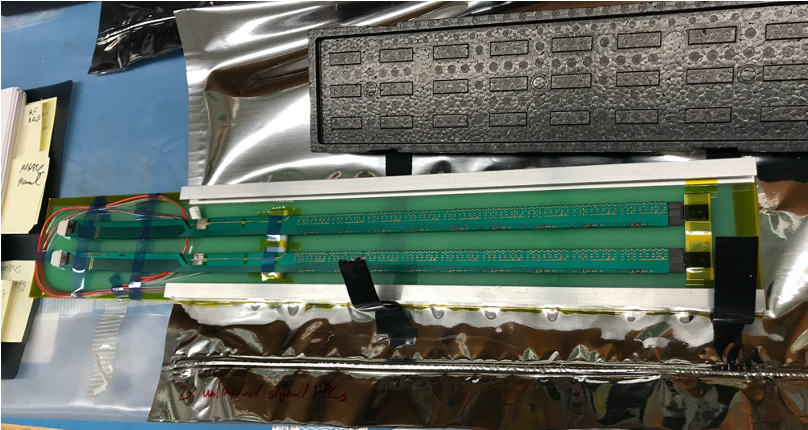
\includegraphics[width=0.9\linewidth]{mvtx_staves}
  \caption{Two of the production MVTX staves.  These are nearly
    identical to the ALICE ITS inner barrel stavs.  The only
    modification is the use of a slightly longer power cable soldered
    to the stave.}
  \label{fig:mvtx_oblique}
\end{figure}

The INTT is a silicon strip detector which surrounds the MVTX
(Fig.~\ref{fig:intt}).  This detector interpolates between the
extremely fine pitch of the MVTX and the slightly coarser spatial
resolution of the TPC.  It is also the only tracking detector with
single event timing resolution --- the ability to uniquely associate
hits with a specific bunch crossing --- and is therefore key to
associating fully reconstructed tracks with the event that produced
them.

\begin{figure}[hbt!]
  \centering
  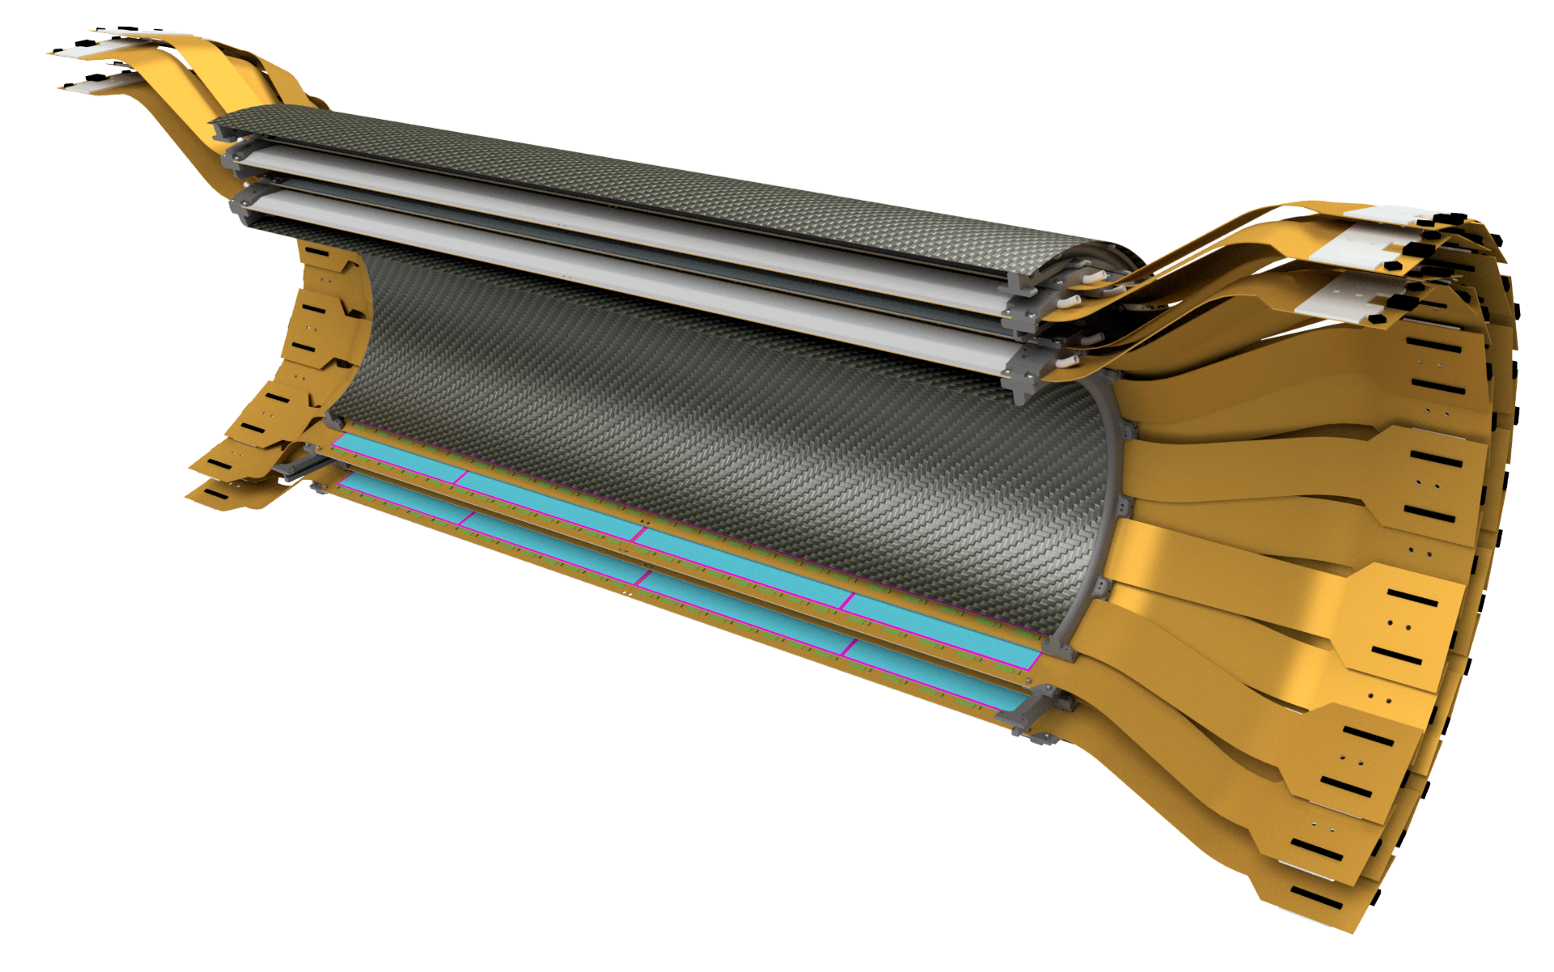
\includegraphics[width=0.9\linewidth]{intt}
  \caption{A rendering of the silicon strip intermediate tracker
    (INTT), being built by RIKEN and NCU Taiwan.  While the sensors
    (blue) are off-the-shelf Hamamatsu parts, the flexible high
    density cables (orange) which carry signals and power have been a
    target of extensive R\&D with industrial partners due to their
    length.}
  \label{fig:intt}
\end{figure}


\begin{figure}[hbt!]
  \centering
  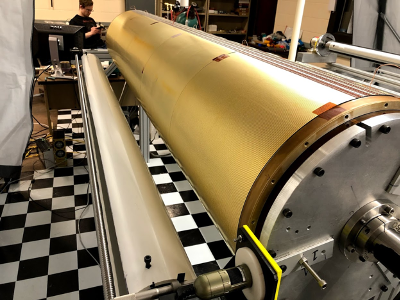
\includegraphics[width=0.49\linewidth]{innerfieldcage}
  \hfill
  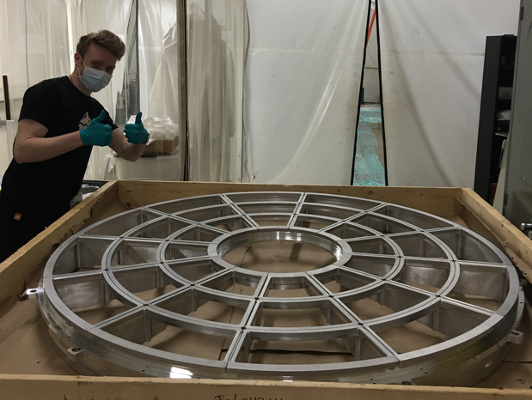
\includegraphics[width=0.49\linewidth]{wagonwheel}
  \caption{(left) The inner field cage of the TPC. A length of PVC
    sewer pipe, milled to a precise outer diameter, was used as an
    economical form upon which the field cage was built.  (right) One
    of the two TPC ``wagon wheels'' which supports the TPC field
    cages, the GEMs, the readout electronics and all the services.
    The wheels are each milled from a single billet of aluminum
    improving the gas tightness of the TPC by eliminating a large
    number of seams.}
  \label{fig:wagonwheel}
\end{figure}

\begin{figure}[hbt!]
  \centering
  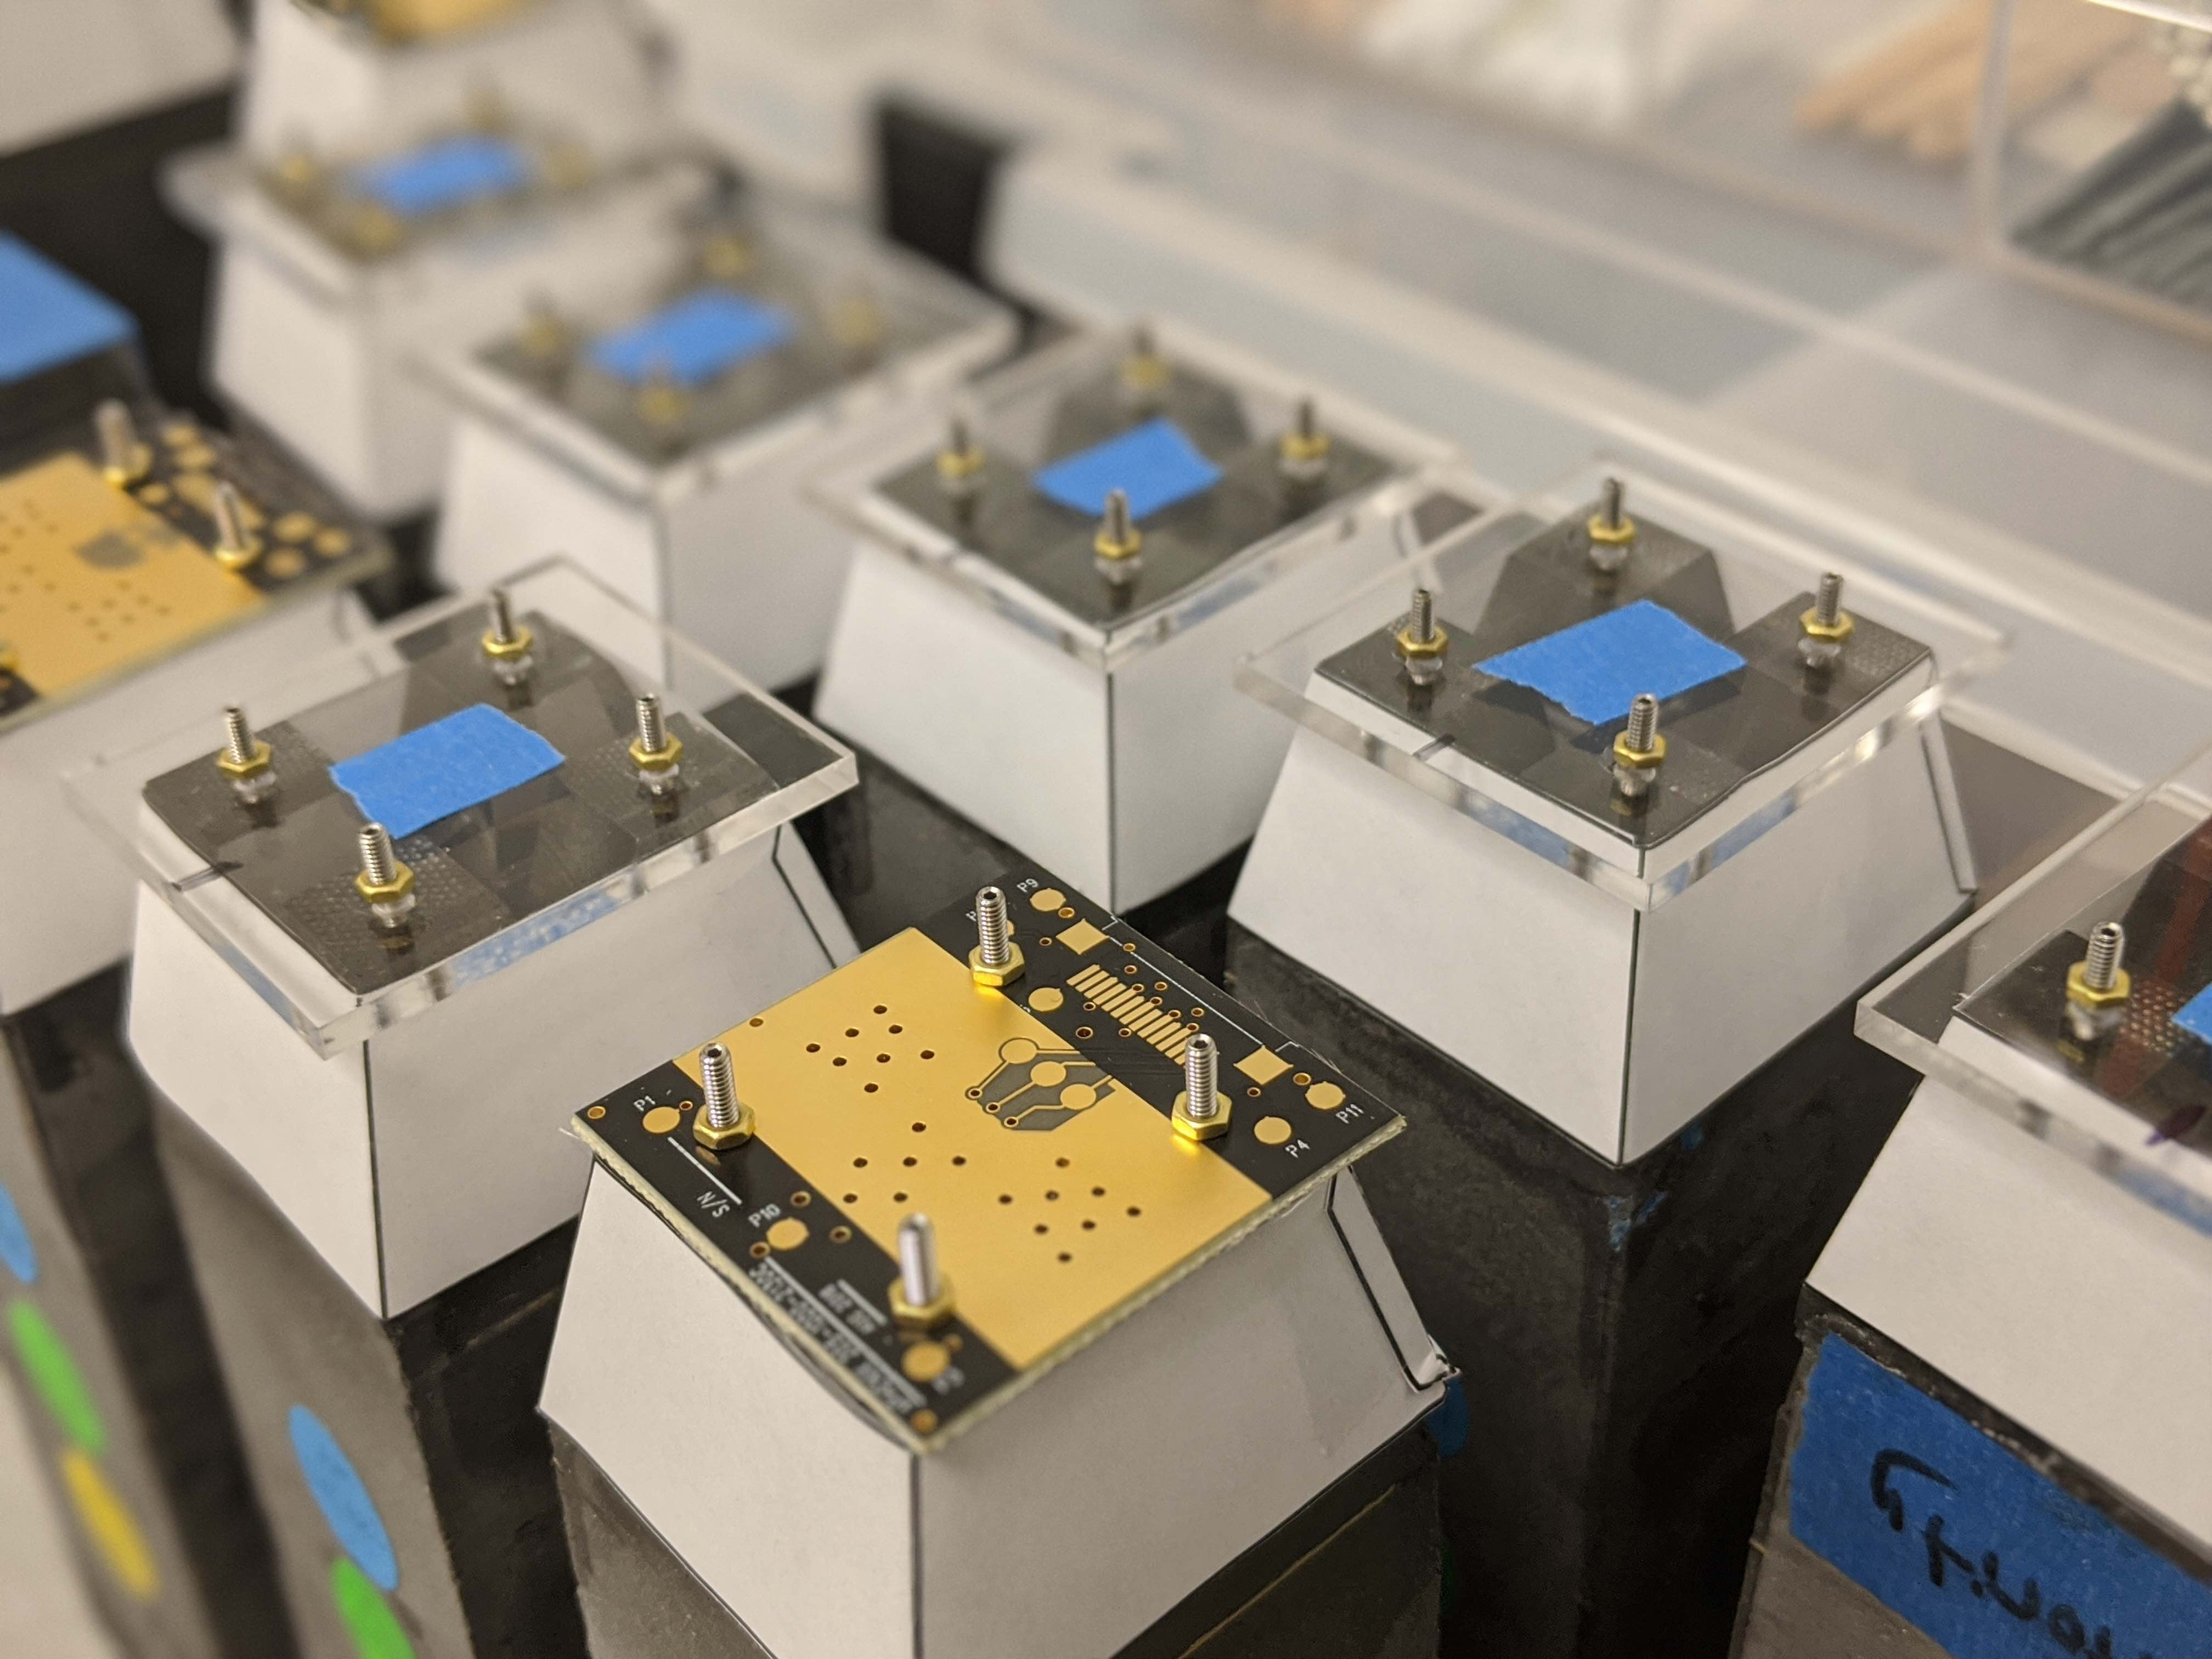
\includegraphics[trim = 0 0 1000 0, clip, width=0.62\linewidth]{emcalblocks}
  \hfill
  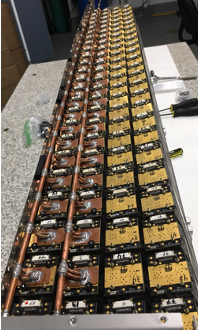
\includegraphics[width=0.37\linewidth]{sector0}
  \caption{The EMCal blocks and the assembled EMCal Sector ``0''.}
  \label{fig:emcal}
\end{figure}

\begin{figure}[hbt!]
  \centering
  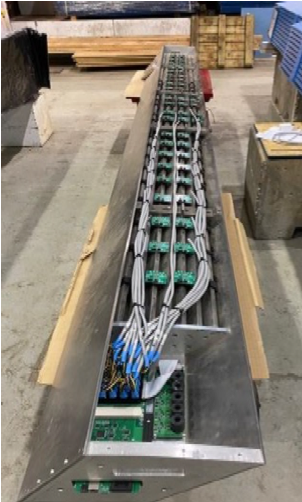
\includegraphics[width=0.42\linewidth]{ihcalsector}
  \hfill
  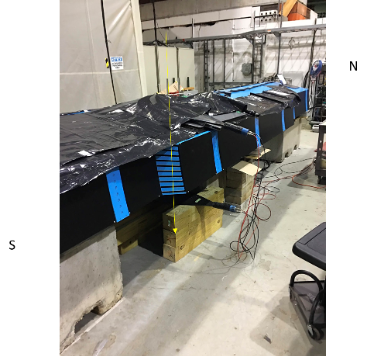
\includegraphics[trim = 20 0 20 0, clip, width=0.56\linewidth]{ohcalsector}
  \caption{Inner and outer HCal sectors.}
  \label{fig:hcal}
\end{figure}

\begin{figure}[hbt!]
  \centering
  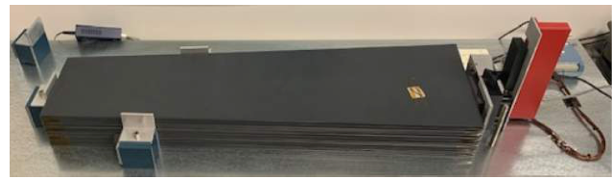
\includegraphics[width=0.75\linewidth]{tiletesting}
  \caption{Testing the HCal tiles at GSU.}
  \label{fig:tiletesting}
\end{figure}

\begin{figure}[hbt!]
  \centering
  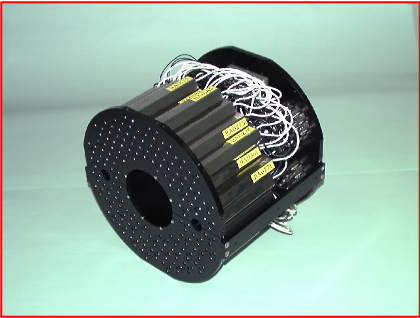
\includegraphics[trim = 5 5 5 5, clip]{mbd}
  \caption{The minimum bias detector, originally built by Hiroshima
    University for PHENIX.}
  \label{fig:mbd}
\end{figure}

\section{Effects of COVID-19}
\label{sec:covid}

The coronavirus pandemic continues to have a significant effects on the
project, though many steps have been taken to mitigate the most severe
impacts.

Project planning anticipated a large effort over the summer of 2020
coming from students and postdocs working on the assembly and testing
of detector components both at BNL and at other Labs and universities.
BNL went into a ``min safe'' mode in late March, which halted nearly
all in person work on the oHCal and EMCal sector assembly.  Similar
stoppages happened at Fudan University and UIUC on EMCal block
production.  These efforts have recently begun to resume, but with
significant changes to work procedures.

The pandemic happened to strike at a time when major aspects of the
project could proceed without needing people to be physically present
at BNL.  Design work and reviews continued.  And some industries, such
as steel manufacturing, had been deemed essential by the US Government
and continued their work with little or no interruption.  The overall
effect on the project has been to use up some schedule float,
tightening the schedule ahead of the early 2023 data taking, but
without endangering the schedule leading to the planned date of PD-4.


\section{Potential relationship to EIC}
\label{sec:eic}

The potential connection between sPHENIX and the EIC experimental
program has a long history.  sPHENIX traces its origin to the October
2009 charge from then ALD Steve Vigdor to the PHENIX collaboration to
detail its plans for the coming decade.  In that charge, he asked
about, ``Any plans or interest your Collaboration has in adapting your
detector or detector subsystems (or detector R\&D) to study
electron-nucleon and electron-ion collisions with an eventual eRHIC
upgrade.''  Subsequent charges from ALD Berndt Mueller have been even
more explicit in asking the potential relevance to be demonstrated
through extensive studies and documentation.  In 2013, the PHENIX
collaboration was asked to develop a ``letter of intent'' for an EIC
detector based on sPHENIX.  In 2018, the sPHENIX collaboration was
asked to revisit this question and produce a ``design study update''.
Among the institutions that make up the sPHENIX scientific
collaboration are a significant number with acknowledged and relevant
physics expertise and interest in the EIC experimental program.  The
sPHENIX project is overseen by the ALD's office, aided by the Project
Management Committee, and sPHENIX project management has met with that
committee at least biweekly for some years, dating back to before
CD-0.  The committee membership has evolved over time but has included
experts on EIC physics and instrumentation, and they have been asked
to keep an eye on the potential reuse of parts of the sPHENIX detector
and its extensively upgraded infrastructure for a possible EIC
detector.

